\section{Imagen de una función de dos variables}

\begin{ejercicio}
    Calcular la imagen de la función $f: A \to \bb{R}$, donde
    \begin{equation*}
        A = \{(x,y)\in \bb{R}^2\mid x^2\leq 2y-y^2\}
        \qquad \text{y} \qquad
        f(x,y)=x^2+y(y^3-4)
    \end{equation*}

    Veamos en primer lugar el conjunto en el que está definido, $A$:
    \begin{equation*}
        \begin{split}
            A &= \{(x,y)\in \bb{R}^2\mid x^2\leq 2y-y^2\}
            = \{(x,y)\in \bb{R}^2\mid x^2- 2y+y^2\leq 0\} =\\
            &= \{(x,y)\in \bb{R}^2\mid x^2 + (y-1)^2\leq 1\} =\\
            &= \ol{B}[(0,1),1]
        \end{split}
    \end{equation*}
    \begin{figure}[H]
        \centering
        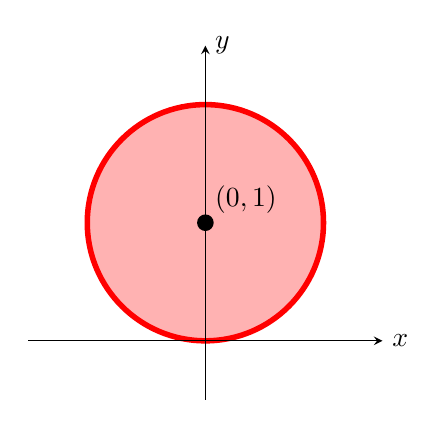
\begin{tikzpicture}[scale=1.5]
            % Círculo
            \draw[fill=red!30, draw=red, line width=2pt] (0,1) circle [radius=1];
            
            % Punto central
            \fill (0,1) circle [radius=2pt] node[above right] {$(0,1)$};

            % Ejes
            \draw[-stealth] (-1.5,0) -- (1.5,0) node[right] {$x$};
            \draw[-stealth] (0,-0.5) -- (0,2.5) node[right] {$y$};
        \end{tikzpicture}
        \caption{Conjunto de definición $A=\ol{B}[(0,1),1]$.}
    \end{figure}

    Como $A$ es una bola cerrada, tenemos que es un conjunto cerrado y acotado, luego compacto. Además, es convexo, luego conexo. Como $f$ es continua por ser polinómica, tenemos que $f(A)\subset \bb{R}$ es compacto (Teorema de Weierstrass) y conexo (Teorema del Valor Intermedio), por lo que es un intervalo cerrado y acotado, por lo que tiene mínimo y máximo.

    Estudiamos en primer lugar su interior. Tenemos que $A^\circ = B[(0,1),1]$. Como $f$ es diferenciable en todo punto de $A^\circ$ por ser polinómica, tenemos que $f$ es parcialmente derivable en todo punto $(x,y)\in A^\circ$, con:
    \begin{equation*}
        \del{f}{x}(x,y) = 2x \\
        \del{f}{y}(x,y) = 4y^3-4
    \end{equation*}
    Por tanto, los puntos críticos del interior de $A$ son aquellos que cumplen la condición necesaria de extremo relativo, $\nabla f(x,y)=0$. En este caso, el único punto crítico del interior de $A$ es el punto $(0,1)\in A^\circ$.

    Nos falta por estudiar la frontera de $A$. Tenemos que:
    \begin{equation*}
        \begin{split}
            \Fr A &= \{(x,y)\in \bb{R}^2\mid x^2= 2y-y^2\}
            =\\
            &= \{(x,y)\in \bb{R}^2\mid x^2 + (y-1)^2= 1\} =\\
            &= S[(0,1),1]
        \end{split}
    \end{equation*}

    Además, como para todo $(x,y)\in A$, se tiene que $x^2 + (y-1)^2\leq 1$, entonces:
    \begin{equation*}
        (y-1)^2\leq 1 \Longrightarrow |y-1|\leq 1 \Longrightarrow y\in [0,2]
    \end{equation*}
    
    Por tanto, para $(x,y)\in \Fr A\subset A$, tenemos que:
    \begin{equation*}
        f(x,y) = x^2+y(y^3-4) = 2y-y^2 + y^4-4y = y^4-y^2-2y
    \end{equation*}

    Es decir, $f(\Fr A)=h([0,2])$, con $h:[0,2]\to \bb{R}$ dada por $h(y)=y^4-y^2-2y$. Calculamos por tanto la imagen de dicha función real de variable real. Como es polinómica, tenemos que $h$ es derivable en $[0,2]$, con $h'(y)=4y^3-2y-2$. Los puntos críticos son entonces los que anulan la primera derivada:
    \begin{figure}[H]
        \centering
        \polyhornerscheme[x=1]{2x^3-x-1}
    \end{figure}
    Por tanto, tenemos que $h'(y)=2(y-1)(2y^2+2y+1)$. Como $y\in [0,2]$, tenemos que el segundo factor no se anula. Por tanto, tenemos que los posibles extremos absolutos de $h$ son $\{0,1,2\}$.
    \begin{equation*}
        h(0)=0 \qquad h(1)=-2 \qquad h(2)=16-4-4 = 8
    \end{equation*}
    Por tanto, $h([0,2])=f(\Fr A) = [-2,8]$.

    Como el único candidato a extremo relativo del interior de $A$ era el punto $(0,1)$, y $f(0,1)=-3$, tenemos que:
    \begin{equation*}
        f(A)=[-3,8]
    \end{equation*}
    El mínimo absoluto se da en $(0,1)$, y el máximo absoluto se da para $y=2$, es decir, para el punto $(0,2)$.
\end{ejercicio}








\begin{ejercicio}
    Calcular la imagen de la función $f: A \to \bb{R}$, donde
    \begin{equation*}
        A = \{(x,y)\in \bb{R}^2\mid (x-1)^2+y^2\leq 4,~x\geq 0\}
        \qquad \text{y} \qquad
        f(x,y)=(x-2)^2+2y^2
    \end{equation*}

    Veamos en primer lugar el conjunto en el que está definido, $A$:
    \begin{equation*}
        \begin{split}
            A &= \{(x,y)\in \bb{R}^2\mid (x-1)^2+y^2\leq 4,~x\geq 0\}
            = \ol{B}[(1,0),2]\cap (\bb{R}^+_0\times \bb{R})
        \end{split}
    \end{equation*}
    \begin{figure}[H]
        \centering
        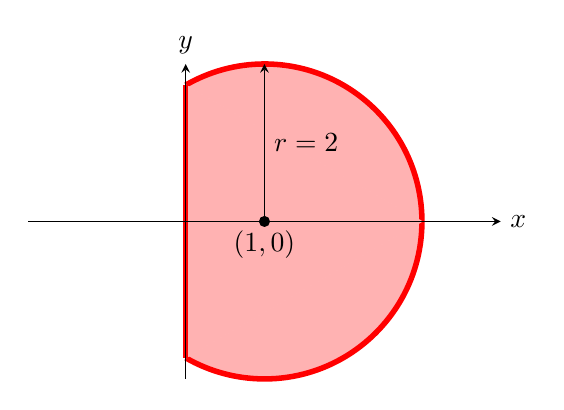
\begin{tikzpicture}
            % Círculo (solo la parte con x positiva)
            \draw[fill=red!30, draw=red, line width=2pt] (3,0) arc (0:120:2);
            \draw[fill=red!30, draw=red, line width=2pt] (3,0) arc (0:-120:2);
            \draw[fill=red!30, draw=red!30] (0,{sqrt(3)}) -- (3,0) -- (0,{-sqrt(3)}) --cycle;
            \draw[red, line width=2pt] (0,{sqrt(3)}) -- (0,{-sqrt(3)});

            % Punto (1,0)
            \fill (1,0) circle [radius=2pt] node[below] {$(1,0)$};

            % Marca en del radio
            \draw[-stealth] (1,0) -- node[right] {$r=2$} (1,2);

            % Ejes
            \draw[-stealth] (-2,0) -- (4,0) node[right] {$x$};
            \draw[-stealth] (0,-2) -- (0,2) node[above] {$y$};
        \end{tikzpicture}
            
        \caption{Conjunto de definición $A$.}
    \end{figure}

    
    Tenemos que $\bb{R}^+_0\times \bb{R}=g^{-1}([0,+\infty[)$, donde $g:\bb{R}\to \bb{R}$ dada por $g(x)=x$ es una función continua y $[0,+\infty[$ es un cerrado. Como la imagen inversa de un cerrado mediante una función continua es un cerrado, tenemos que $\bb{R}^+_0\times \bb{R}$ es un cerrado. Además, como una bola cerrada es un cerrado, tenemos que $A$ es la intersección de dos cerrados, luego es cerrado. Además, es acotado, ya que $A\subset B[(1,0), 3]$ (por ejemplo). Por tanto como es cerrado y acotado y $A\subset \bb{R}^n$, tenemos que es compacto. 

    Además, una bola cerrada es convexa, y el semiplano $x\geq 0$ también es convexo, luego su intersección es convexa, luego conexa. 
    
    Como $f$ es continua por ser polinómica, tenemos que $f(A)\subset \bb{R}$ es compacto (Teorema de Weierstrass) y conexo (Teorema del Valor Intermedio), por lo que es un intervalo cerrado y acotado, por lo que tiene mínimo y máximo.

    Estudiamos en primer lugar su interior. Tenemos que $A^\circ = B[(1,0),2]\cap (\bb{R}^+\times \bb{R})$. Como $f$ es diferenciable en todo punto de $A^\circ$ por ser polinómica, tenemos que $f$ es parcialmente derivable en todo punto $(x,y)\in A^\circ$, con:
    \begin{equation*}
        \del{f}{x}(x,y) = 2(x-2) \hspace{2cm}
        \del{f}{y}(x,y) = 4y
    \end{equation*}
    Por tanto, los puntos críticos del interior de $A$ son aquellos que cumplen la condición necesaria de extremo relativo, $\nabla f(x,y)=0$. En este caso, el único punto crítico del interior de $A$ es el punto $(2,0)\in A^\circ$.

    Nos falta por estudiar la frontera de $A$. Tenemos que $\Fr A = C_1 \cup C_2$, donde:
    \begin{equation*}
        \begin{split}
            C_1 &= \{(x,y)\in \bb{R}^2\mid (x-1)^2+y^2= 4,~x\geq 0\}
            =S[(1,0),2]\cap (\bb{R}^+_0\times \bb{R}) \\
            C_2 &= \{(x,y)\in \bb{R}^2\mid x= 0,~(x-1)^2+y^2\leq 4\} = 
            \{(0,y)\in \bb{R}^2\mid 1^2+y^2\leq 4\} = \\
            &\quad =\{(0,y)\in \bb{R}^2\mid y^2\leq 3\} = 
            \left\{(0,y)\in \bb{R}^2\mid y \in [-\sqrt{3}, \sqrt{3}]\right\}
        \end{split}
    \end{equation*}

    Estudiamos en primer lugar $C_1$. En este arco paramétrico, tenemos que $y^2 = 4-(x-1)^2$.
    Además, como en todo punto de $C_1$ se tiene que $(x-1)^2\leq 4,~x\geq 0$, tenemos que $|x-1|\leq 2,~x\geq 0$, luego $x\in [0,3]$.
    Definimos entonces la siguiente función auxiliar:
    \Func{h_1}{[0,3]}{\bb{R}^2}{x}{(x-2)^2 + 2y^2 = (x-2)^2 + 2(4-(x-1)^2)}
    Tenemos que $h_1$ es una función real de variable real. Como es polinómica, es derivable en todo punto de
    $]0,3[$, por lo que los puntos críticos de su interior son aquellos que anulan la primera derivada:
    \begin{multline*}
        h_1(x) = (x-2)^2 + 2(4-(x-1)^2) = x^2+4-4x + 8 - 2x^2 - 2 +4x = -x^2+10
        \Longrightarrow \\ \Longrightarrow
        h_1'(x) = -2x = 0 \Longleftrightarrow x=0
    \end{multline*}

    Por tato, tenemos que los candidatos a extremos absolutos de $h_1$ son $\{0,3\}$.
    \begin{equation*}
        h_1(0)=10 \qquad h_1(3)=1
    \end{equation*}
    Por tanto, $h_1([0,3])=f(C_1) = [1,10]$.


    Estudiamos ahora $C_2$. En este caso, nos definimos la siguiente función auxiliar:
    \Func{h_2}{[-\sqrt{3},\sqrt{3}]}{\bb{R}^2}{y}{(x-2)^2 + 2y^2 = 4 + 2y^2}
    Tenemos que $h_2$ es una función real de variable real. Como es polinómica, es derivable en todo punto de
    $]-\sqrt{3},\sqrt{3}[$, por lo que los puntos críticos de su interior son aquellos que anulan la primera derivada:
    \begin{equation*}
        h_2'(y) = 4y = 0 \Longleftrightarrow y=0
    \end{equation*}
    Por tanto, tenemos que los candidatos a extremos absolutos de $h_2$ son $\{-\sqrt{3},0,\sqrt{3}\}$.
    \begin{equation*}
        h_2(-\sqrt{3})=h_2(\sqrt{3})=10 \qquad h_2(0)=4
    \end{equation*}
    Por tanto, $h_2([-\sqrt{3},\sqrt{3}])=f(C_2) = [4,10]$.

    Como el único candidato a extremo relativo del interior de $A$ era el punto $(2,0)$, y $f(2,0)=0$, tenemos que:
    \begin{equation*}
        f(A)=[0,10]
    \end{equation*}
\end{ejercicio}

\begin{ejercicio}
    Calcular la imagen de la función $f: A \to \bb{R}$, donde
    \begin{equation*}
        A = \{(x,y)\in \bb{R}^2\mid 2x^2+y^2\leq 2\}
        \qquad \text{y} \qquad
        f(x,y)=x^2(y-1)^3
    \end{equation*}

    Veamos en primer lugar el conjunto en el que está definido, $A$:
    \begin{equation*}
        A = \left\{(x,y)\in \bb{R}^2\mid x^2+\frac{y^2}{2}\leq 1\right\}
    \end{equation*}
    Por tanto, se trata de una elipse centrada en el origen,
    con semiejes $b=1$ y $a=\sqrt{2}$, con el eje mayor en el eje $Y$.
    \begin{figure}[H]
        \centering
        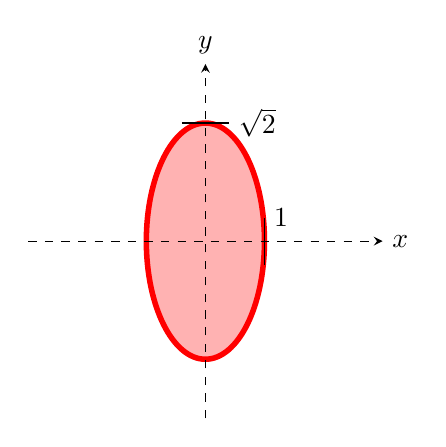
\begin{tikzpicture}[scale=1.5]
            % Elipse
            \draw[fill=red!30, draw=red, line width=2pt] (0,0) ellipse (0.5 and 1);
            % Ejes
            \draw[-stealth, dashed] (-1.5,0) -- (1.5,0) node[right] {$x$};
            \draw[-stealth, dashed] (0,-1.5) -- (0,1.5) node[above] {$y$};
            % Marcas
            \draw (0.5,-0.2) -- (0.5,0.2) node[right] {$1$};
            \draw (-0.2,1) -- (0.2,1) node[right] {$\sqrt{2}$};
        \end{tikzpicture}
        \caption{Conjunto de definición $A$.}
    \end{figure}

    Sabemos que $A$ es homeomorfo a $\ol{B}(0,1)$, por lo que es compacto y conexo. 
    No obstante, resolveremos dicho ejercicio sin usar dicha propiedad, parte del temario de Topología I.
    
    En primer lugar, sabemos que es cerrado, ya que es la imagen inversa mediante una función polinómica (luego continua)
    del intervalo $]-\infty,1]$, que es cerrado. Además, es acotado, ya que $A\subset B(0, 2)$ (por ejemplo). Por tanto como es cerrado y acotado y $A\subset \bb{R}^n$, tenemos que es compacto.

    Para ver que es conexo, vamos a ver que es convexo. Sea $(x_1,y_1), (x_2,y_2)\in A$. Tenemos que ver que $[(x_1,y_1), (x_2,y_2)]\subset A$.
    En efecto, un punto de dicho segmento es de la forma:
    \begin{equation*}
        (1-t)(x_1,y_1)+t(x_2,y_2) = ((1-t)x_1+tx_2, (1-t)y_1+ty_2) \qquad \text{con } t\in [0,1]
    \end{equation*}
    Por tanto, tenemos que:
    \begin{equation*}
        \begin{split}
            2((1-t)x_1&+tx_2)^2 + ((1-t)y_1+ty_2)^2
            \stackrel{(\ast)}{\leq}
            2((1-t)x_1^2+tx_2^2) + ((1-t)y_1^2+ty_2^2)
            =\\&= (1-t)[2x_1^2+y_1^2] + t[2x_2^2+y_2^2]
            \stackrel{(\ast\ast)}{\leq} (1-t)\cdot 2 + t\cdot 2 = 2
            \qquad \forall t\in [0,1]
        \end{split}
    \end{equation*}
    donde en $(\ast)$ hemos usado que, como la función
    $g:\bb{R}\to \bb{R}$ dada por $g(x)=x^2$ es convexa, entonces
    $[(1-t)a + tb]^2 \leq (1-t)a^2 + tb^2$ para todo $a,b\in \bb{R}$ y todo $t\in [0,1]$.
    En $(\ast\ast)$ hemos usado que $(x_1,y_1), (x_2,y_2)\in A$.
    Por tanto, tenemos que $[(x_1,y_1), (x_2,y_2)]\subset A$, luego $A$ es convexo, luego conexo.

    Como $f$ es continua por ser polinómica, tenemos que $f(A)\subset \bb{R}$ es compacto (Teorema de Weierstrass) y conexo (Teorema del Valor Intermedio), por lo que es un intervalo cerrado y acotado, por lo que tiene mínimo y máximo.

    Estudiamos en primer lugar su interior. Tenemos que $A^\circ = \{(x,y)\in \bb{R}^2\mid 2x^2+y^2< 2\}$. Como $f$ es diferenciable en todo punto de $A^\circ$ por ser polinómica, tenemos que $f$ es parcialmente derivable en todo punto $(x,y)\in A^\circ$, con:
    \begin{equation*}
        \del{f}{x}(x,y) = 2x(y-1)^3 \hspace{2cm}
        \del{f}{y}(x,y) = 3x^2(y-1)^2
    \end{equation*}

    Por tanto, los puntos críticos del interior de $A$ son aquellos que cumplen la condición necesaria de extremo relativo, $\nabla f(x,y)=0$.
    \begin{equation*}
        \nabla f(x,y) = (0,0) \Longleftrightarrow
        \begin{cases}
            2x(y-1)^3 = 0 \\
            3x^2(y-1)^2 = 0
        \end{cases}
        \Longleftrightarrow
        \begin{cases}
            x=0 \\
            \quad \lor \\
            y=1
        \end{cases}
    \end{equation*}

    Por tanto, hay un conjunto no numerable de puntos críticos del interior de $A$. Estos son $\{(0,y), (x,1)\in \bb{R}^2\mid x,y\in \bb{R}\}$. Tenemos que:
    \begin{equation*}
        f(0,y) = 0 \qquad f(x,1) = 0
    \end{equation*}

    Nos falta por estudiar la frontera de $A$. Tenemos que $\Fr A = \{(x,y)\in \bb{R}^2\mid 2x^2+y^2= 2\}$. Tenemos que $x^2 = 1-\frac{y^2}{2}$.
    Además, como en todo punto de $A$, se tiene que $y^2\leq 2$, por lo que $y\in \left[-\sqrt{2},\sqrt{2}\right]$. Nos definimos entonces la siguiente función auxiliar:
    \Func{h}{\left[-\sqrt{2},\sqrt{2}\right]}{\bb{R}}{y}{x^2(y-1)^3 = \left(1-\dfrac{y^2}{2}\right)(y-1)^3}

    Tenemos que $h$ es una función real de variable real. Como es polinómica, es derivable en todo punto de $]-\sqrt{2},\sqrt{2}[$, por lo que los puntos críticos de su interior son aquellos que anulan la primera derivada:
    \begin{multline*}
        h'(y) = -y(y-1)^3 + \left(1-\dfrac{y^2}{2}\right)[3(y-1)^2]
        = (y-1)^2\left[-y(y-1) + 3\left(1-\dfrac{y^2}{2}\right)\right]
        =\\= (y-1)^2\left[-y^2 + y + 3 - \dfrac{3y^2}{2}\right]
        = (y-1)^2\left[-\dfrac{5y^2}{2} + y + 3\right]
        = 0 \Longleftrightarrow
        \begin{cases}
            y=1 \\
            \quad \lor \\
            y=\dfrac{1\pm \sqrt{31}}{5}
        \end{cases}
    \end{multline*}
    Veamos cuáles valores de $y$ son válidos. Como $y\in \left[-\sqrt{2},\sqrt{2}\right]$, tenemos que:
    \begin{gather*}
        \dfrac{1\pm\sqrt{31}}{5} < \sqrt{2} \Longleftrightarrow 1 \pm \sqrt{31} < 5\sqrt{2} \Longleftrightarrow 1 + 31 \pm 2\sqrt{31} < 50 \Longleftrightarrow \pm \sqrt{31} < 18 \\
        \dfrac{1\pm\sqrt{31}}{5} > \sqrt{-2} \Longleftrightarrow 1 \pm \sqrt{31} >- 5\sqrt{2} \Longleftrightarrow -1 \mp \sqrt{31} < 5\sqrt{2} \Longleftrightarrow \\ \hspace{4cm} \Longleftrightarrow 1 + 31 \pm 2\sqrt{31} < 50 \Longleftrightarrow \pm \sqrt{31} <18
    \end{gather*}

    Por tanto, tenemos que los tres candidatos son válidos. Veamos cuáles son los extremos absolutos de $h$ en $\left[-\sqrt{2},\sqrt{2}\right]$.
    \begin{equation*}
        h\left(\sqrt{2}\right) = h\left(-\sqrt{2}\right) = 0 = h(1)
    \end{equation*}
    Por la complejidad de los cálculos, evitamos calcular la imagen de los otros dos puntos críticos, sino tan solo su signo.
    Como $h(y)= \left(1-\dfrac{y^2}{2}\right)(y-1)^3$ y el primer término siempre es positivo, el segundo término, $y-1$, determina el signo de $h(y)$.
    \begin{gather*}
        h\left(\frac{1+\sqrt{31}}{5}\right) > 0 \Longleftrightarrow
        \frac{1+\sqrt{31}}{5} > 1 \Longleftrightarrow
        1+\sqrt{31} > 5 \Longleftrightarrow
        \sqrt{31} > 4 \Longleftrightarrow 31 > 16 \\
        h\left(\frac{1-\sqrt{31}}{5}\right) < 0 \Longleftrightarrow
        \frac{1-\sqrt{31}}{5} < 1 \Longleftrightarrow
        1-\sqrt{31} < 5 \Longleftrightarrow
        -\sqrt{31} < 4
    \end{gather*}
    Por tanto, tenemos que la imagen de $f$ es:
    \begin{equation*}
        f(A) = \left[h\left(\frac{1-\sqrt{31}}{5}\right), h\left(\frac{1+\sqrt{31}}{5}\right)\right]
    \end{equation*}
\end{ejercicio}

\begin{ejercicio}
    Calcular la imagen de la función $f: A \to \bb{R}$, donde
    \begin{equation*}
        A = \{(x,y)\in \bb{R}^2\mid 0\leq x \leq 2-y^2\}
        \qquad \text{y} \qquad
        f(x,y)=x^2+y^2 -2x
    \end{equation*}

    Veamos en primer lugar el conjunto en el que está definido, $A$:
    \begin{align*}
        A &= \{(x,y)\in \bb{R}^2\mid x\geq 0\} \cap \{(x,y)\in \bb{R}^2\mid x\leq 2-y^2\}
    \end{align*}
    El primer conjunto es directo ver que se trata del semiplano $x\geq 0$. El segundo conjunto es
    la región del plano delimitada por la parábola $x=-y^2+2$. Dibujémoslo:
    \begin{figure}[H]
        \centering
        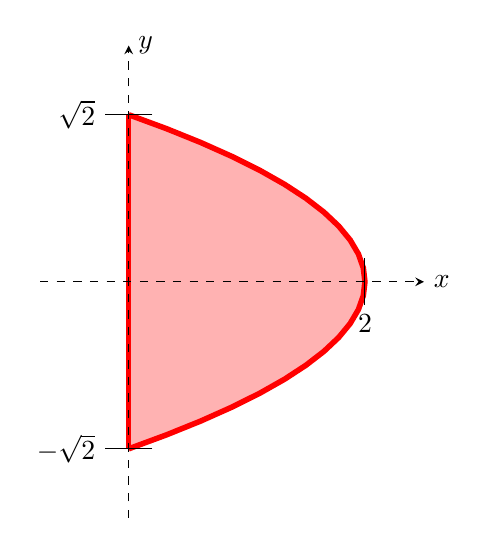
\begin{tikzpicture}[scale=1.5]

            % Raiz de 2
            \pgfmathsetmacro{\raiz}{sqrt(2)}

            % Parábola
            \draw[fill=red!30, draw=red, line width=2pt] plot[domain=-\raiz:\raiz] ({-\x*\x+2}, \x);

            % Cierre con el eje Y
            \draw[fill=red!30, draw=red, line width=2pt] (0,\raiz) -- (0,-\raiz) -- cycle;

            % Ejes
            \draw[-stealth, dashed] (-0.75,0) -- (2.5,0) node[right] {$x$};
            \draw[-stealth, dashed] (0,-2) -- (0,2) node[right] {$y$};
            % Marcas
            \draw (0.2,\raiz) -- (-0.2,\raiz) node[left] {$\sqrt{2}$};
            \draw (0.2,-\raiz) -- (-0.2,-\raiz) node[left] {$-\sqrt{2}$};
            \draw (2, 0.2) -- (2, -0.2) node[below] {$2$};
        \end{tikzpicture}
        \caption{Conjunto de definición $A$.}
    \end{figure}

    Sabemos que $A$ es homeomorfo a $\ol{B}(0,1)$, por lo que es compacto y conexo.
    No obstante, resolveremos dicho ejercicio sin usar dicha propiedad, parte del temario de Topología I.

    En primer lugar, sabemos que el semiplano $x\geq 0$ es cerrado, ya que es la imagen inversa mediante una función polinómica (luego continua) del intervalo $[0,+\infty[$, que es cerrado.
    La región delimitada por la parábola es cerrada, ya que es la imagen inversa mediante una función polinómica (luego continua) del intervalo $]-\infty,2]$, que es cerrado.
    Por tanto, $A$ es la intersección de dos cerrados, luego es cerrado.
    
    Además, es acotado, ya que $A\subset B(0, 7)$ (por ejemplo). Por tanto como es cerrado y acotado y $A\subset \bb{R}^n$, tenemos que es compacto. Veamos ahora que es conexo.
    El semiplano es convexo. Veamos que la región delimitada por la parábola también lo es. Sea $P$ dicha región,
    y sean $(x_1,y_1), (x_2,y_2)\in P$. Tenemos que ver que $[(x_1,y_1), (x_2,y_2)]\subset P$.
    Un punto de dicho segmento es de la forma:
    \begin{equation*}
        (1-t)(x_1,y_1)+t(x_2,y_2) = ((1-t)x_1+tx_2, (1-t)y_1+ty_2) \qquad \text{con } t\in [0,1]
    \end{equation*}

    Por tanto, tenemos que:
    \begin{equation*}
        \begin{split}
            \left((1-t)y_1+ty_2\right)^2 &+ \left((1-t)x_1+tx_2\right)
            \stackrel{(\ast)}{\leq}
            (1-t)y_1^2 + ty_2^2 + (1-t)x_1 + tx_2
            = \\ &= (1-t)[y_1^2 + x_1] + t[y_2^2 + x_2]
            \stackrel{(\ast\ast)}{\leq} (1-t)\cdot 2 + t\cdot 2
            = 2\cdot (1-t+t) = 2
        \end{split}
    \end{equation*}
    donde en $(\ast)$ hemos usado que, como la función $g:\bb{R}\to \bb{R}$ dada por $g(x)=x^2$ es convexa, entonces $[(1-t)a + tb]^2 \leq (1-t)a^2 + tb^2$ para todo $a,b\in \bb{R}$ y todo $t\in [0,1]$.
    En $(\ast\ast)$ hemos usado que $(x_1,y_1), (x_2,y_2)\in P$. Por tanto, tenemos que $[(x_1,y_1), (x_2,y_2)]\subset P$, luego $P$ es convexo.

    Como la intersección de dos conjuntos convexos es convexa, tenemos que $A$ es convexo, luego conexo.

    Por tanto, tenemos que $A$ es compacto y conexo, y como $f\in C^1(A)$, en particular continua, tenemos que
    $f(A)\subset \bb{R}$ es compacto (Teorema de Weierstrass) y conexo (Teorema del Valor Intermedio), por lo que es un intervalo cerrado y acotado, por lo que tiene mínimo y máximo. Es decir:
    \begin{equation*}
        f(A) = [\min f(A), \max f(A)]
    \end{equation*}

    Estudiamos en primer lugar su interior. Tenemos que: $$A^\circ = \{(x,y)\in \bb{R}^2\mid 0< x < 2-y^2\}$$
    Como $f$ es diferenciable en todo punto de $A^\circ$ por ser polinómica, tenemos que $f$ es parcialmente derivable en todo punto $(x,y)\in A^\circ$, con:
    \begin{equation*}
        \del{f}{x}(x,y) = 2x-2 \hspace{2cm}
        \del{f}{y}(x,y) = 2y
    \end{equation*}
    
    Por tanto, los puntos críticos del interior de $A$ son aquellos que
    cumplen la condición necesaria de extremo relativo, $\nabla f(x,y)=0$. En este caso, el único punto crítico del interior de $A$ es el punto $(1,0)\in A^\circ$,
    con $f(1,0)=-1$.

    Nos falta por estudiar la frontera de $A$. Tenemos que:
    \begin{equation*}
        \Fr A = \{(x,y)\in \bb{R}^2\mid x=0, x+y^2\leq 2\} \cup \{(x,y)\in \bb{R}^2\mid x=2-y^2, x\geq 0\}
    \end{equation*}

    Sea $C_1=\{(x,y)\in \bb{R}^2\mid x=0, x+y^2\leq 2\}=\{(0,y)\in \bb{R}^2\mid y^2\leq 2\}$.
    Además, como en $C_1$ se tiene $x=0$, $f_{\big| C_1}(y)=y^2$. Nos definimos entonces la siguiente función auxiliar:
    \Func{h_1}{\left[-\sqrt{2},\sqrt{2}\right]}{\bb{R}}{y}{x^2 +y^2 -2x = y^2}

    Tenemos que $h_1$ es una función real de variable real. Como es polinómica, es derivable en todo punto de $]-\sqrt{2},\sqrt{2}[$, por lo que los puntos críticos de su interior son aquellos que anulan la primera derivada:
    \begin{equation*}
        h_1'(y) = 2y = 0 \Longleftrightarrow y=0
    \end{equation*}
    Por tanto, tenemos que los candidatos a extremos absolutos de $h_1$ son $\{-\sqrt{2},0,\sqrt{2}\}$.
    \begin{equation*}
        h_1(-\sqrt{2})=h_1(\sqrt{2})=2 \qquad h_1(0)=0
    \end{equation*}
    Por tanto, $h_1\left(\left[-\sqrt{2},\sqrt{2}\right]\right)=f(C_1) = [0,2]$.

    Sea $C_2=\{(x,y)\in \bb{R}^2\mid x=2-y^2, x\geq 0\}$. Para todo punto de $x$, se tiene que $x\geq 0$, luego $2-y^2\geq 0$, luego $y^2\leq 2$.
    Por tanto, en $C_2$, como $x=2-y^2$ y $0\leq y^2\leq 2$, tenemos que $x\in [0,2]$. Por tanto, definimos la siguiente función auxiliar:
    \Func{h_2}{\left[0,2\right]}{\bb{R}}{x}{x^2 +y^2 -2x = x^2 + 2-x - 2x = x^2 -3x +2}

    Tenemos que $h_2$ es una función real de variable real. Como es polinómica, es derivable en todo punto de $]0,2[$, por lo que los puntos críticos de su interior son aquellos que anulan la primera derivada:
    \begin{equation*}
        h_2'(x) = 2x -3 = 0 \Longleftrightarrow x=\frac{3}{2}
    \end{equation*}
    Por tanto, tenemos que los candidatos a extremos absolutos de $h_2$ son $\{-\sqrt{2},\nicefrac{3}{2},\sqrt{2}\}$.
    \begin{equation*}
        h_2(0)=2 \qquad h_2(2)=0 \qquad h_2\left(\frac{3}{2}\right) = -\frac{1}{4}
    \end{equation*}

    Por tanto, $h_2\left(\left[0,2\right]\right)=f(C_2) = \left[-\frac{1}{4}, 2\right]$. Por tanto, tenemos que la imagen de $f$ es:
    \begin{equation*}
        f(A) = \left[-1, 2\right]
    \end{equation*}
\end{ejercicio}
    

\begin{ejercicio}
    Calcular la imagen de la función $f: A \to \bb{R}$, donde
    \begin{equation*}
        A = \{(x,y)\in \bb{R}^2\mid -1 \leq x \leq y \leq 1\}
        \qquad \text{y} \qquad
        f(x,y)=x^2+y^2 +xy -x
    \end{equation*}

    Veamos en primer lugar el conjunto en el que está definido, $A$:
    \begin{equation*}
        A = \{(x,y)\in \bb{R}^2\mid x\geq -1\} \cap \{(x,y)\in \bb{R}^2\mid y\leq 1\} \cap \{(x,y)\in \bb{R}^2\mid x-y \leq 0\}
    \end{equation*}

    \begin{figure}[H]
        \centering
        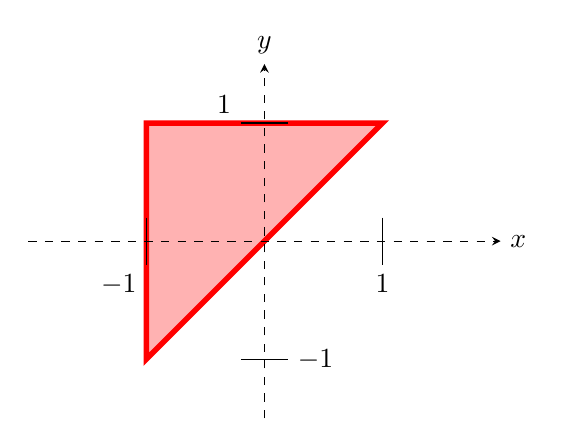
\begin{tikzpicture}[scale=1.5]
            % Recta
            \draw[fill=red!30, draw=red, line width=2pt] (-1,-1) -- (1,1) -- (-1,1) -- cycle;
            
             % Ejes
             \draw[-stealth, dashed] (-2,0) -- (2,0) node[right] {$x$};
             \draw[-stealth, dashed] (0,-1.5) -- (0,1.5) node[above] {$y$};
             
             % Marcas
            \draw (-1,0.2) -- (-1,-0.2) node[below left] {$-1$};
            \draw (1,0.2) -- (1,-0.2) node[below] {$1$};
            \draw (0.2,1) -- (-0.2,1) node[above left] {$1$};
            \draw (-0.2,-1) -- (0.2,-1) node[right] {$-1$};
        \end{tikzpicture}
        \caption{Conjunto de definición $A$.}
    \end{figure}

    Se trata de tres conjuntos cerrados, ya que son la imagen inversa mediante funciones polinómicas (luego continuas) de $[-1,+\infty[$, $]-\infty,1]$ y $]-\infty,0]$, respectivamente.
    Por tanto, $A$ es la intersección de tres cerrados, luego es cerrado. Además, es acotado, ya que $A\subset B(0, 2)$ (por ejemplo). Por tanto como es cerrado y acotado y $A\subset \bb{R}^n$, tenemos que es compacto. Veamos ahora que es conexo.

    Tenemos que en los tres casos se trata de semiplanos, por lo que son convexos. Como
    la intersección de convexos es convexa, tenemos que $A$ es convexo, luego conexo.

    Por tanto, tenemos que $A$ es compacto y conexo, y como $f\in C^1(A)$, en particular continua, tenemos que $f(A)\subset \bb{R}$ es compacto (Teorema de Weierstrass) y conexo (Teorema del Valor Intermedio), por lo que es un intervalo cerrado y acotado, por lo que tiene mínimo y máximo. Es decir:
    \begin{equation*}
        f(A) = [\min f(A), \max f(A)]
    \end{equation*}

    Estudiamos en primer lugar su interior. Tenemos que: $$A^\circ = \{(x,y)\in \bb{R}^2\mid -1< x < y < 1\}$$
    Como $f$ es diferenciable en todo punto de $A^\circ$ por ser polinómica, tenemos que $f$ es parcialmente derivable en todo punto $(x,y)\in A^\circ$, con:
    \begin{equation*}
        \del{f}{x}(x,y) = 2x+y-1 \hspace{2cm}
        \del{f}{y}(x,y) = 2y+x
    \end{equation*}

    Por tanto, los puntos críticos del interior de $A$ son aquellos que cumplen la condición necesaria de extremo relativo,
    $\nabla f(x,y)=0$. En este caso, el único punto que anula el gradiente es el punto $(\nicefrac{2}{3},\nicefrac{-1}{3})$, pero este punto no pertenece al interior de $A$,
    por lo que no es candidato a extremo relativo del interior de $A$.

    Nos falta por estudiar la frontera de $A$. Tenemos que $\Fr A = C_1\cup C_2\cup C_3$, donde:
    \begin{align*}
        C_1 &= \{(x,y)\in \bb{R}^2\mid x=-1, -1\leq y \leq 1\} \\
        C_2 &= \{(x,y)\in \bb{R}^2\mid y=1, -1\leq x \leq 1\} \\
        C_3 &= \{(x,y)\in \bb{R}^2\mid x-y = 0, -1\leq x \leq 1\}
    \end{align*}

    Estudiamos en primer lugar $C_1$. Definimos la siguiente función auxiliar:
    \Func{h_1}{[-1,1]}{\bb{R}}{y}{(-1)^2 +y^2 +(-1)y -(-1) = y^2 -y+2}

    Tenemos que $h_1$ es una función real de variable real. Como es polinómica, es derivable en todo punto de $]-1,1[$, por lo que los puntos críticos de su interior son aquellos que anulan la primera derivada:
    \begin{equation*}
        h_1'(y) = 2y -1 = 0 \Longleftrightarrow y=\frac{1}{2}
    \end{equation*}
    Por tanto, tenemos que los candidatos a extremos absolutos de $h_1$ son $\{-1,\nicefrac{1}{2},1\}$.
    \begin{equation*}
        h_1(-1)=4 \qquad h_1(1)=2 \qquad h_1\left(\frac{1}{2}\right) = \frac{7}{4}
    \end{equation*}

    Por tanto, $h_1([-1,1])=f(C_1) = \left[\nicefrac{7}{4}, 4\right]$. Estudiamos en segundo lugar $C_2$. Definimos la siguiente función auxiliar:
    \Func{h_2}{[-1,1]}{\bb{R}}{x}{x^2 +1 +x -x = x^2 +1}

    Tenemos que $h_2$ es una función real de variable real. Como es polinómica, es derivable en todo punto de $]-1,1[$, por lo que los puntos críticos de su interior son aquellos que anulan la primera derivada:
    \begin{equation*}
        h_2'(x) = 2x = 0 \Longleftrightarrow x=0
    \end{equation*}
    Por tanto, tenemos que los candidatos a extremos absolutos de $h_2$ son $\{-1,0,1\}$.
    \begin{equation*}
        h_2(-1)=h(1)=2 \qquad h_2(0) = 1
    \end{equation*}

    Por tanto, $h_2([-1,1])=f(C_2) = [1,2]$. Estudiamos en tercer lugar $C_3$. Definimos la siguiente función auxiliar:
    \Func{h_3}{[-1,1]}{\bb{R}}{x}{x^2 +x^2 +x^2-x = 3x^2-x}

    Tenemos que $h_3$ es una función real de variable real. Como es polinómica, es derivable en todo punto de $]-1,1[$, por lo que los puntos críticos de su interior son aquellos que anulan la primera derivada:
    \begin{equation*}
        h_3'(x) = 6x -1 = 0 \Longleftrightarrow x=\frac{1}{6}
    \end{equation*}

    Por tanto, tenemos que los candidatos a extremos absolutos de $h_3$ son $\{-1,\nicefrac{1}{6},1\}$.
    \begin{equation*}
        h_3(-1)=4 \qquad h_3(1)=2 \qquad h_3\left(\frac{1}{6}\right) = -\frac{1}{12}
    \end{equation*}

    Por tanto, $h_3([-1,1])=f(C_3) = \left[\nicefrac{-1}{12}, 4\right]$. Por tanto, tenemos que la imagen de $f$ es:
    \begin{equation*}
        f(A) = \left[-\frac{1}{12},4\right]
    \end{equation*}
\end{ejercicio}


\begin{ejercicio}[Prueba DGIIM 2022-23 y 2023-24\footnote{Se repitió ambos años.}]
    Calcular la imagen de la función $f:A\to \bb{R}$, donde
    \begin{equation*}
        A = \{(x,y)\in \bb{R}^2\mid 0\leq x \leq 2(1-y^2)\}
        \qquad \text{y} \qquad
        f(x,y)=(x-1)^4 + y^2
    \end{equation*}

    Veamos en primer lugar el conjunto en el que está definido, $A$:
    \begin{align*}
        A &= \{(x,y)\in \bb{R}^2\mid x\geq 0\} \cap \{(x,y)\in \bb{R}^2\mid x+2y^2\leq 2\}
    \end{align*}

    El primer conjunto es directo ver que se trata del semiplano $x\geq 0$. El segundo conjunto es
    la región del plano delimitada por la parábola $x=-2y^2+2$. Dibujémoslo:
    \begin{figure}[H]
        \centering
        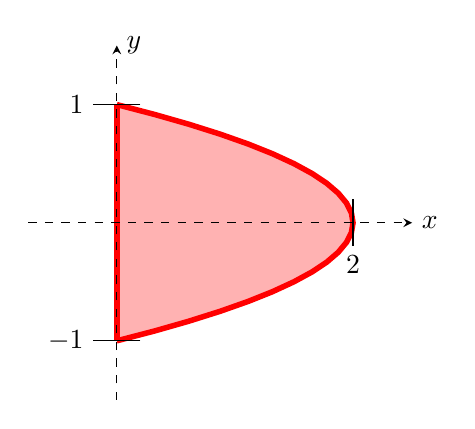
\begin{tikzpicture}[scale=1.5]

            % Parábola
            \draw[fill=red!30, draw=red, line width=2pt] plot[domain=-1:1] ({-2*\x*\x+2}, \x);

            % Cierre con el eje Y
            \draw[fill=red!30, draw=red, line width=2pt] (0,1) -- (0,-1) -- cycle;

            % Ejes
            \draw[-stealth, dashed] (-0.75,0) -- (2.5,0) node[right] {$x$};
            \draw[-stealth, dashed] (0,-1.5) -- (0,1.5) node[right] {$y$};
            % Marcas
            \draw (0.2,1) -- (-0.2,1) node[left] {${1}$};
            \draw (0.2,-1) -- (-0.2,-1) node[left] {$-{1}$};
            \draw (2, 0.2) -- (2, -0.2) node[below] {$2$};
        \end{tikzpicture}
        \caption{Conjunto de definición $A$.}
    \end{figure}

    Sabemos que $A$ es homeomorfo a $\ol{B}(0,1)$, por lo que es compacto y conexo.
    No obstante, resolveremos dicho ejercicio sin usar dicha propiedad, parte del temario de Topología I.

    En primer lugar, sabemos que el semiplano $x\geq 0$ es cerrado, ya que es la imagen inversa mediante una función polinómica (luego continua) del intervalo $[0,+\infty[$, que es cerrado.
    La región delimitada por la parábola es cerrada, ya que es la imagen inversa mediante una función polinómica (luego continua) del intervalo $]-\infty,2]$, que es cerrado.
    Por tanto, $A$ es la intersección de dos cerrados, luego es cerrado.
    
    Además, es acotado, ya que $A\subset B(0, 7)$ (por ejemplo). Por tanto como es cerrado y acotado y $A\subset \bb{R}^n$, tenemos que es compacto. Veamos ahora que es conexo.
    El semiplano es convexo. Veamos que la región delimitada por la parábola también lo es. Sea $P$ dicha región,
    y sean $(x_1,y_1), (x_2,y_2)\in P$. Tenemos que ver que $[(x_1,y_1), (x_2,y_2)]\subset P$.
    Un punto de dicho segmento es de la forma:
    \begin{equation*}
        (1-t)(x_1,y_1)+t(x_2,y_2) = ((1-t)x_1+tx_2, (1-t)y_1+ty_2) \qquad \text{con } t\in [0,1]
    \end{equation*}

    Por tanto, tenemos que:
    \begin{equation*}
        \begin{split}
            \left((1-t)x_1+tx_2\right) &+ 2\left((1-t)y_1+ty_2\right)^2
            \stackrel{(\ast)}{\leq}
            (1-t)x_1+tx_2 + 2\left((1-t)y_1^2 + ty_2^2\right) =
            \\&= (1-t)\left(x_1 + 2y_1^2\right) + t\left(x_2 + 2y_2^2\right)
            \stackrel{(\ast\ast)}{\leq} (1-t)\cdot 2 + t\cdot 2 = 2
        \end{split}
    \end{equation*}
    donde en $(\ast)$ hemos usado que, como la función $g:\bb{R}\to \bb{R}$ dada por $g(x)=x^2$ es convexa, entonces $[(1-t)a + tb]^2 \leq (1-t)a^2 + tb^2$ para todo $a,b\in \bb{R}$ y todo $t\in [0,1]$.
    En $(\ast\ast)$ hemos usado que $(x_1,y_1), (x_2,y_2)\in P$. Por tanto, tenemos que $[(x_1,y_1), (x_2,y_2)]\subset P$, luego $P$ es convexo. Como la intersección de dos conjuntos convexos es convexa, tenemos que $A$ es convexo, luego conexo.

    Por tanto, tenemos que $A$ es compacto y conexo, y como $f\in C^1(A)$, en particular continua, tenemos que
    $f(A)\subset \bb{R}$ es compacto (Teorema de Weierstrass) y conexo (Teorema del Valor Intermedio), por lo que es un intervalo cerrado y acotado, por lo que tiene mínimo y máximo. Es decir:
    \begin{equation*}
        f(A) = [\min f(A), \max f(A)]
    \end{equation*}

    Estudiamos en primer lugar su interior. Tenemos que: $$A^\circ = \{(x,y)\in \bb{R}^2\mid 0< x < 2-2y^2\}$$
    Como $f$ es diferenciable en todo punto de $A^\circ$ por ser polinómica, tenemos que $f$ es parcialmente derivable en todo punto $(x,y)\in A^\circ$, con:
    \begin{equation*}
        \del{f}{x}(x,y) = 4(x-1)^3 \hspace{2cm}
        \del{f}{y}(x,y) = 2y
    \end{equation*}
    
    Por tanto, los puntos críticos del interior de $A$ son aquellos que
    cumplen la condición necesaria de extremo relativo, $\nabla f(x,y)=0$. En este caso, el único punto crítico del interior de $A$ es el punto $(1,0)\in A^\circ$,
    con $f(1,0)=0$.

    Nos falta por estudiar la frontera de $A$. Tenemos que:
    \begin{equation*}
        \Fr A = \{(x,y)\in \bb{R}^2\mid x=0, x+2y^2\leq 2\} \cup \{(x,y)\in \bb{R}^2\mid x=2-2y^2, x\geq 0\}
    \end{equation*}

    Sea $C_1=\{(x,y)\in \bb{R}^2\mid x=0, x+2y^2\leq 2\}=\{(0,y)\in \bb{R}^2\mid y^2\leq 1\}$.
    Nos definimos entonces la siguiente función auxiliar:
    \Func{h_1}{\left[-1,1\right]}{\bb{R}}{y}{(x-1)^4+y^2 = 1+y^2}

    Tenemos que $h_1$ es una función real de variable real. Como es polinómica, es derivable en todo punto de $]-1,1[$, por lo que los puntos críticos de su interior son aquellos que anulan la primera derivada:
    \begin{equation*}
        h_1'(y) = 2y = 0 \Longleftrightarrow y=0
    \end{equation*}
    Por tanto, tenemos que los candidatos a extremos absolutos de $h_1$ son $\{-1,0,1\}$.
    \begin{equation*}
        h_1(-1)=h_1(1)=2 \qquad h_1(0)=1
    \end{equation*}
    Por tanto, $h_1\left(\left[-1,1\right]\right)=f(C_1) = [1,2]$.

    Sea $C_2=\{(x,y)\in \bb{R}^2\mid x=2-2y^2, x\geq 0\}$. Como $2-2y^2\geq 0$, tenemos que $y\in \left[-1,1\right]$, por lo que $y^2\in [0,1]$. Además, como en $C_2$ se tiene $x=2-2y^2$, se tiene que $y^2=1-\frac{x}{2}$ y $x\in [0,2]$. Por tanto, definimos la siguiente función auxiliar:
    \Func{h_2}{\left[0,2\right]}{\bb{R}}{x}{(x-1)^4+y^2 = (x-1)^4 + 1-\frac{x}{2}}

    Tenemos que $h_2$ es una función real de variable real. Como es polinómica, es derivable en todo punto de $]-1,1[$, por lo que los puntos críticos de su interior son aquellos que anulan la primera derivada:
    \begin{equation*}
        h_2'(x) = 4(x-1)^3 - \frac{1}{2} = 0 \Longleftrightarrow x=\frac{3}{2}
    \end{equation*}
    Por tanto, tenemos que los candidatos a extremos absolutos de $h_2$ son $\{0,\nicefrac{3}{2},2\}$.
    \begin{equation*}
        h_2(0)=2 \qquad h_2(2)=1 \qquad h_2\left(\frac{3}{2}\right) = \frac{5}{16}
    \end{equation*}

    Por tanto, $h_2\left(\left[0,2\right]\right)=f(C_2) = \left[\frac{5}{16}, 2\right]$. Por tanto, tenemos que la imagen de $f$ es:
    \begin{equation*}
        f(A) = \left[0, 2\right]
    \end{equation*}
\end{ejercicio}


\begin{ejercicio}[Ordinaria DGIIM 2023-24]
    Calcula la imagen de la función $f:A\to \bb{R}$, donde
    \begin{equation*}
        A = \{(x,y)\in \bb{R}^2\mid x^2+y^2\leq 1,~y\geq 0\}
        \qquad \text{y} \qquad
        f(x,y)=\frac{xy}{2+x^2+y^2}
    \end{equation*}
\end{ejercicio}



\begin{ejercicio}[Ordinaria DGIIM 2022-23]
    Calcula la imagen de la función $f:A\to \bb{R}$, donde
    \begin{equation*}
        A = \{(x,y)\in \bb{R}^2\mid x^2+y^2\leq 1\}
        \qquad \text{y} \qquad
        f(x,y)=\frac{xy}{1+x^2+y^2}
    \end{equation*}

    Veamos en primer lugar el conjunto en el que está definido, $A$:
    \begin{figure}[H]
        \centering
        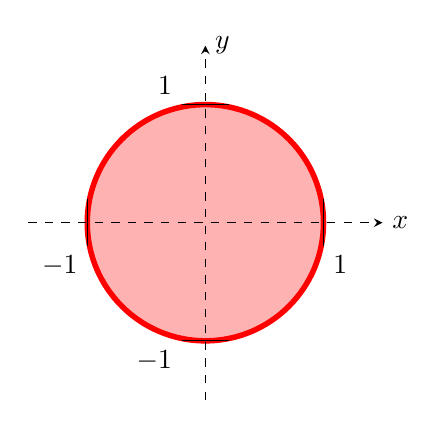
\begin{tikzpicture}[scale=1.5]
            % Circunferencia
            \draw[fill=red!30, draw=red, line width=2pt] (0,0) circle (1);
            
            % Ejes
            \draw[-stealth, dashed] (-1.5,0) -- (1.5,0) node[right] {$x$};
            \draw[-stealth, dashed] (0,-1.5) -- (0,1.5) node[right] {$y$};
            
            % Marcas
            \draw (0.2,1) -- (-0.2,1) node[above left] {$1$};
            \draw (0.2,-1) -- (-0.2,-1) node[below left] {$-1$};
            \draw (1, 0.2) -- (1, -0.2) node[below right] {$1$};
            \draw (-1, 0.2) -- (-1, -0.2) node[below left] {$-1$};
        \end{tikzpicture}
        \caption{Conjunto de definición $A$.}
    \end{figure}

    Sabemos que $A$ es una bola cerrada, por lo que es un conjunto
    cerrado y acotado, luego es compacto. Además, como es una bola,
    es convexo, luego es conexo. Por tanto, tenemos que $A$ es compacto y conexo, y como $f\in C^1(A)$ por ser racional,
    en particular es continua y tenemos que $f(A)\subset \bb{R}$ es compacto (Teorema de Weierstrass) y conexo (Teorema del Valor Intermedio), por lo que es un intervalo cerrado y acotado, por lo que tiene mínimo y máximo. Es decir:
    \begin{equation*}
        f(A) = [\min f(A), \max f(A)]
    \end{equation*}

    Estudiamos en primer lugar su interior. Tenemos que: $$A^\circ = \{(x,y)\in \bb{R}^2\mid x^2+y^2< 1\}=B(0,1)$$
    Como $f$ es diferenciable en todo punto de $A^\circ$ por ser racional, tenemos que $f$ es parcialmente derivable en todo punto $(x,y)\in A^\circ$, con:
    \begin{equation*}
        \del{f}{x}(x,y) = \frac{y(1+x^2+y^2) - xy(2x)}{(1+x^2+y^2)^2} = \frac{y(1-x^2+y^2)}{(1+x^2+y^2)^2} \qquad \forall (x,y)\in A^\circ
    \end{equation*}

    Por simetría, tenemos que:
    \begin{equation*}
        \del{f}{y}(x,y) = \frac{x(1-y^2+x^2)}{(1+x^2+y^2)^2} \qquad \forall (x,y)\in A^\circ
    \end{equation*}

    Por tanto, los puntos críticos del interior de $A$ son aquellos que cumplen la condición necesaria de extremo relativo,
    $\nabla f(x,y)=0$. En este caso, los puntos críticos del interior de $A$ son los puntos $(x,y)\in A^\circ$ tales que $y=0$ o $x=0$.
    \begin{equation*}
        \left\{
            \begin{array}{l}
                y(1-x^2+y^2) = 0 \\
                x(1-y^2+x^2) = 0
            \end{array}
        \right.
    \end{equation*}
    Como $x^2+y^2<1$, tenemos que $x^2<1$. Por tanto, tenemos que $1-x^2+y^2 > 1-x^2> 0$,
    luego la primera ecuación solo se da para $y=0$. Análogamente, la segunda ecuación solo se da para $x=0$.
    Por tanto, el único punto crítico del interior de $A$ es el punto $(0,0)\in A^\circ$, con $f(0,0)=0$.

    Nos falta por estudiar la frontera de $A$. Tenemos que $\Fr A = S(0,1)$, la circunferencia unidad centrada en el origen, que
    podemos parametriar como:
    \begin{equation*}
        \Fr A = \{(x,y)\in \bb{R}^2\mid x=\cos t, y=\sen t, t\in [-\pi,\pi]\}
    \end{equation*}
    Para $(x,y)=(\cos t, \sen t)$, tenemos que:
    \begin{equation*}
        f(\cos t, \sen t) = \frac{\cos t \sen t}{1+\cos^2 t + \sen^2 t} = \frac{\cos t \sen t}{2} = \frac{\sen 2t}{4}
    \end{equation*}

    Por tanto, nos definimos la siguiente función auxiliar:
    \Func{h}{[-\pi,\pi]}{\bb{R}}{t}{\frac{\sen 2t}{4}}

    Tenemos que $h$ es una función real de variable real. Como es polinómica, es derivable en todo punto de $]-\pi,\pi[$, por lo que los puntos críticos de su interior son aquellos que anulan la primera derivada:
    \begin{equation*}
        h'(t) = \frac{2\cos 2t}{4} = 0 \Longleftrightarrow \cos 2t = 0
    \end{equation*}
    Usando que $t\in [-\pi,\pi]$, tenemos que los puntos que anulan $h'$ son $\{-\nicefrac{\pi}{4},\nicefrac{\pi}{4},\nicefrac{3\pi}{4},-\nicefrac{3\pi}{4}\}$.
    Por tanto, tenemos que los candidatos a extremos absolutos de $h$ son $\{\pm\pi,\pm\nicefrac{\pi}{4},\pm\nicefrac{3\pi}{4}\}$. Tenemos que:
    \begin{equation*}
        h(-\pi)=h(\pi)=0 \qquad h\left(\frac{\pi}{4}\right)=h\left(\frac{3\pi}{4}\right)=\frac{1}{4}
        \qquad 
        h\left(-\frac{\pi}{4}\right)=h\left(-\frac{3\pi}{4}\right)=-\frac{1}{4}
    \end{equation*}

    Por tanto, $h\left(\left[-\pi,\pi\right]\right)=f(\Fr A) = \left[-\frac{1}{4}, \frac{1}{4}\right]$. Por tanto, tenemos que la imagen de $f$ es:
    \begin{equation*}
        f(A) = \left[-\frac{1}{4},\frac{1}{4}\right]
    \end{equation*}
\end{ejercicio}



\begin{ejercicio}[Ordinaria DGIIM 2023-24 Incidencias]
    Calcula la imagen de la función $f:A\to \bb{R}$, donde
    \begin{equation*}
        A = \{(x,y)\in \bb{R}^2\mid x^2+y^2\leq 1,~y\geq 0\}
        \qquad \text{y} \qquad
        f(x,y)=x^2+y^2-x-y
    \end{equation*}
\end{ejercicio}